\chapter{离散数学}{

\section{前置知识}

\section{集合论}{

\subsection{集合论的主要内容}{
  \begin{itemize}
    \item 研究对象 : 集合,关系,函数,自然数,基数
    \item 研究思想 : 以逻辑为基础,以集合为工具,表示和构造各种数学对象
    \item 研究内容 : \begin{itemize}
            \item 集合的基本概念 : 集合之间的关系,运算,恒等式
            \item 二元关系 : 表示,性质,函数,等价关系,序关系
            \item 自然数 : 皮亚诺系统,自然数的运算,性质
            \item 基数 : 有序集于无穷集,基数的比较
            \item 良序,超限归纳法
          \end{itemize}
  \end{itemize}
}%集合论的主要内容结尾

\subsection{集合论中的问题}{
  \begin{itemize}
    \item 如何给集合下定义?
    \item 如何用集合去定义关系,函数,自然数?
    \item 如何比较集合的大小?
    \item 能否把每个集合的元素依次列举出来?
    \item 有没有最大的集合?
  \end{itemize}
}%集合论中的问题结尾

\subsection{集合的表示}{
  \begin{itemize}
    \item {
          列举法 :

          列出集合中的全体元素,元素之间用逗号分开,然后用花括号括起来,比如 : $A = \{a,b,c,d\},B = \{2,4,6,\dots\}$.
          }
    \item {
          描述法 :

          用谓词$P(x)$表示$x$具有性质$P$,用$\{x | P(x)\}$表示具有性质$P$的集合.例如 : $P_1(x)$表示$x$是英文字母,$P_2(x)$表示$x$是十进制数字,$C = \{x | P_1(x)\}$表示26个英文字母的集合,$D = \{x | P_2(x)\}$表示10个十进制数字的集合.
          }
  \end{itemize}
}%集合的表示结尾

\subsection{描述集合的注意事项}{
  \begin{enumerate}
    \item 集合中的元素是各不相同的.
    \item 集合中的元素不规定顺序.
    \item {
          集合的两种表示法可以互相转化,例如,$B={2,4,6,...}$可用描述法表示为$B=\{x|x>0\mbox{且x是偶数}\}$或$B=\{x|x=2(k+1),\mbox{k为非负整数}\}$.
          }
  \end{enumerate}
}%描述集合的注意事项结尾

\subsection{常用的集合}{
  \begin{itemize}
    \item $\mathNatureNumberCollection$: 自然数集合 $\mathNatureNumberCollection = {0,1,2,3,\dots}$
    \item $\mathIntegerCollection$: 整数集合 $\mathIntegerCollection = {0, \pm 1, \pm 2, \dots} = {\dots, -2, -1, 0, 1, 2, \dots}$
    \item $\mathRationalNumberCollection$: 有理数集合
    \item $\mathRealNumberCollection$: 实数集合
    \item $\mathComplexNumberCollection$: 复数集合
  \end{itemize}
}%常用的集合结尾

\subsection{集合之间的关系}{

\subsubsection{子集}{
  设$A,B$为二集合,若$B$中的元素都是$A$中的元素,则称$B$是$A$的子集,也称$A$包含$B$,或者$B$包含于$A$,记作$B \subseteq A$,其符号化形式为 : $$
    B \subseteq A \Leftrightarrow \forall x (x \in B \to x \in A)
  $$
  若$B$不是$A$的子集,则记作$B \subsetneq A$,其符号化形式为 : $$
    B \subsetneq A \Leftrightarrow \exists x (x \in B \land x \notin A)
  $$
}%子集结尾

\subsubsection{有限集和无限集}{
  \begin{itemize}
    \item 有限集,即元素数量优先的集合,定义叙述为 : $S$是由$n$个元素组成的集合($n$是非负正整数,包含0),则称$S$为有限集.
    \item 无限集:不是有限集的集合都是无限集.
  \end{itemize}
}%有限集和无限集结尾

\subsubsection{可列集}{
  可列集是无限集的一种,如果某无限集$S$中的元素可以按某种规则排成一列,并且无重复,无遗漏,则称该$S$为可列集.

  此时$S$可以被用列举法或者描述法表示.

  任何无限集都包含可列集,但是无限集本身不一定是可列集.

  另外,可列个可列集的并也是可列集.

}%可列集结尾

\subsubsection{相等}{
  设$A,B$为二集合,若$A$包含$B$且$B$包含$A$,则称$A$与$B$相等,记作$A = B$,符号化形式为 : $$
    A = B \Leftrightarrow \forall x (x \in B \leftrightarrow x \in A)
  $$
}%相等结尾

\subsubsection{集合之间包含关系的性质}{
  设$A,B,C$为三个集合,则以下三命题为真 :

  \begin{enumerate}
    \item $A \subseteq A$;
    \item 若$A \subseteq A$且$A \neq B$,则$B \subsetneq A$;
    \item 若$A \subseteq B$且$B \subseteq C$,则$A \subseteq C$
  \end{enumerate}
}%集合之间包含关系的性质结尾

\subsubsection{真子集}{
  设$A,B$为二集合,若$A$为$B$的子集且$A \neq B$,则称$A$为$B$的真子集,或者又称$B$真包含$A$,记作$A \subset B$,符号化形式为 : $$
    A \subset B \Leftrightarrow A \subseteq B \land A \neq B
  $$
  若$A$不是$B$的真子集,则记作$A \notRealSubset B$,其符号化形式为 : $$
    A \notRealSubset B \Leftrightarrow \exists x (x \in A \land x \notin B) \land A \neq B
  $$

  设$A,B,C$为三个集合,则以下命题为真 :

  \begin{enumerate}
    \item $A \notRealSubset A$;
    \item 若$A \subset B$,则$B \notRealSubset A$;
    \item 若$A \subset B$,且$B \subset C$,则$A \subset C$
  \end{enumerate}
}%真子集结尾

\subsubsection{空集}{
  不拥有任何元素的集合称为空集合,简称空集,记作$\emptyset$(读作ugh)

  比如$\{x | x^2 + 1 = 0 \land x \in \mathRealNumberCollection\}$和$\{(x,y) | x^2+y^2 < 0 \land x,y \in \mathRealNumberCollection\}$都是空集.

  注意 :

  \begin{itemize}
    \item 空集是一切集合的子集,
    \item 空集是唯一的
    \item 空集是最小的集合.
  \end{itemize}
}%空集结尾

\subsubsection{全集}{
  如果限定所讨论的集合都是某个集合的子集,则称该集合为全集,记作$\mathEverythingCollection$.

  从定义可以看出,全集是相对的,视具体情况而定,因此不唯一.

  比如 : 讨论区间$(a,b)$上的实数的性质时,可以取$(a,b)$为全集,也可以取$[a,b),(a,b],(a , +\infty),\mathRealNumberCollection$等为全集.

  给定若干个集合之后,都可以找到包含它们的全集.在今后讨论中,所涉及的集合都可以看成是某个全集$\mathEverythingCollection$的子集.
}%全集结尾

\subsubsection{集合的元素个数/集合的基数/集合的势}{
  $\emptyset$为$0$元集,含1个元素的集合为单元集或1元集,含两个元素的集合为2元集,依次类推,含$n$个元素的集合称为$n$元集$(n \geq 1)$.

  一个集合$A$所包含的元素数目称为该集合的基数或势(cardinality).记作$\absoluteValue{A}$或者$\#A$或$card(A)$

  当$A$中的元素个数为有限数时($\absoluteValue{A} < \infty$),$A$称为有穷集或有限集,否则称为无限集或者无穷集.
}%集合的元素个数结尾

\subsubsection{幂集}{
  设$A$为一个集合,称由$A$的全体子集组成的集合为$A$的幂集,记作$\powerSetOf{A}$.

  用描述法可以表示为 $\powerSetOf{A} = \{x | x \subseteq A\}$

  注意 :

  \begin{itemize}
    \item 在概率论中也会用$\powerSetOf{A}$来表示事件$A$的概率,两者虽然不相同但是定义是一样的.
    \item 为了避免混淆,也可以用$2^A$表示$A$的幂集.
    \item 这并不是没有道理,设集合$A$的元素个数$\absoluteValue{A} = n$,则$\absoluteValue{\powerSetOf{A}} = 2^n$
  \end{itemize}
}%幂集结尾s

\subsubsection{求幂集的步骤}{
  为了求出给定集合$A$的幂集,先求$A$的由低到高的所有子集,再将它们组成集合.

  设$A = \{a,b,c\}$,求$\powerSetOf{A}$的步骤如下 :

  0元子集为$\emptyset$;1元子集为$\{a\},\{b\},\{c\}$;2元子集为$\{a,b\},\{a,c\},\{b,c\}$;3元子集为$\{a,b,c\} = A$;

  所以,$A$的幂集为 : $$
    \powerSetOf{A} = \{\emptyset,\{a\},\{b\},\{c\},\{a,b\},\{a,c\},\{b,c\},\{a,b,c\}\}
  $$
}%求全集的步骤结尾

\subsubsection{集族}{
除了幂集$\powerSetOf{A}$以外,还有其他形式的由集合构成的集合,统称为集族.若集族中的集合都赋予记号,则可得带指标集的集族.

设$\mathcal{A}$为一个集族,$S$为一个集合,若对于任意的$\alpha \in S$,存在唯一的$A_\alpha \in \mathcal{A}$与之对应,而且$\mathcal{A}$中的任意集合都对应$S$中的某一元素,则称$\mathcal{A}$是以$S$为指标集的集族,$S$称为$\mathcal{A}$的指标集.记为$\mathcal{A} = \{A_\alpha | \alpha \in S\}$,或$\mathcal{A} = \{A_\alpha\}_{\alpha \in S}$

如果把$\emptyset$看作集族,则称$\emptyset$为空集族.
}%集族结尾

\subsubsection{多重集}{
  设全集为$\mathEverythingCollection$,$\mathEverythingCollection$中元素可以不止一次在$A$中出现的集合$A$称为多重集.若$\mathEverythingCollection$中元素$a$在$A$中出现$k$次($k \geq 0$),则称$a$在$A$中重复度为$k$.

  例如 : 设全集$E = \{a,b,c,d,e\},A = \{a,a,b,b,c\}$为多重集,其中$a,b$的重复度为2,$c$的重复度为1,而$d,e$的重复度为0.

  集合可以看作重复度均$\leq 1$的多重集.
}%多重集结尾

}%集合之间的关系结尾

\subsection{集合的运算}{

  \subsubsection{并集}{
    设$A,B$为二集合,称由$A$和$B$的所有元素组成的集合为$A$与$B$的并集,记作$A \unionSet B$,称$\unionSet$为并元算符.

    $A \unionSet B$得到的集合,用描述法可以表示为 : $$
      A \unionSet B = \{x | x \in A \lor x \in B\}
    $$
    集合的并运算可以推广到有限个或可数个集合(初级并).

    设$A_1,A_2,\dots,A_n$为$n$个集合,$A_1,A_2,\dots,A_n,\dots$为可数个集合,则 : $$
      A_1 \unionSet A_2 \unionSet \dots \unionSet A_n = \{x | \exists i (1 \leq i \leq n \land x \in A_i)\}
    $$

    并集也可以写作类似求和的形式 : $$
      \updownUnion{n}{i = 1}A_i = A_1 \unionSet A_2 \unionSet \dots \unionSet A_n
    $$

  }%并集结尾

  \subsubsection{交集}{
    设$A,B$为二集合,称由$A$和$B$的公共元素组成的集合为$A$与$B$的交集,记作$A \intersectionSet B$,称$\intersectionSet$为并元算符.

    $A \intersectionSet B$的描述法表示为$$
      A \intersectionSet B = \{x | x \in A \land x \in B\}
    $$
    集合的交运算可以推广到有限个或可数个集合(初级交).

    设$A_1,A_2,\dots,A_n,\dots$为可数个集合,则 : $$
      A_1 \intersectionSet A_2 \intersectionSet \dots \intersectionSet A_n = \{x | \forall i (1 \leq i \leq n \to x \in A_i)\}
    $$

    同样的,也有这种简化形式 : $$
      \bigcap\limits_{i = 1}^{n}A_i = A_1 \intersectionSet A_2 \intersectionSet \dots \intersectionSet A_n
    $$
  }%交集结尾

  \subsubsection{不相交}{
    设$A,B$为二集合,若$A \intersectionSet B = \emptyset$,则称$A$和$B$是不交的.设$A_1,A_2,\dots$是可数个集合秒如果对于任意的$i \neq j$,都有$A_i \intersectionSet A_j = \neq$,则称$A_1,A_2,\dots$是互不相交的.

    设$A_n = \{x \in R | n - 1 < x < n\},n = 1,2,\dots$,则$A_1,A_2,\dots$是互不相交的.
  }%不相交结尾

  \subsubsection{相对补集}{
    设$A,B$为二集合,称属于$A$而不属于$B$的全体元素组成的集合为$B$对$A$的相对补集,记作$A - B$或$\complement_A B$.$A - B$的描述法表示为 : $$
      A - B = \{x | x \in A \land x \notin B\}
    $$
  }%相对补集

  \subsubsection{对称差}{
    设$A,B$为二集合,称属于$A$而不属于$B$,或属于$B$而不属于$A$的全体元素组成的集合为$A$与$B$的对称差,记作$A \oplus B$.

    $A \oplus B$的描述法表示为 : $$
      A \oplus B = \{x | (x \in A \land x \notin B) \lor (x \notin A \land x \in B)\}
    $$
    容易看出 : $$
      A \oplus B = (A - B) \unionSet (B - A) = (A \unionSet B) - (A \intersectionSet B)
    $$
  }%对称差结尾

  \subsubsection{绝对补集}{
    设$\mathEverythingCollection$为全集,$A \subseteq \mathEverythingCollection$, 称$A$对$\mathEverythingCollection$的相对补集为$A$的绝对补集,记作$A\absoluteCompletementSet$或${~}^\sim A$或$\complement_{\mathEverythingCollection} A$.

    $A\absoluteCompletementSet$的描述法表示为 : $$
      A\absoluteCompletementSet = \{x | x \in \mathEverythingCollection \land x \notin A\}
    $$
    因为$\mathEverythingCollection$是全集,所以$x \in \mathEverythingCollection$是真命题,于是 : $$
      A\absoluteCompletementSet = \{x | x \notin A\}
    $$
  }%绝对补集结尾

  \subsubsection{广义并集}{
    设$\mathcal{A}$为一个集族,称由$\mathcal{A}$中全体元素的元素组成的集合为$\mathcal{A}$的广义并,记作$\bigcup \mathcal{A}$("大并$\mathcal{A}$").

    $\bigcup \mathcal{A}$的描述法表示为 : $$
      \bigcup\mathcal{A} = \{x | \exists z (x \in z \land z \in \mathcal{A})\}
    $$

    设$\mathcal{A} = \{\{a,b\},\{c,d\},\{d,e,f\}\}$,则$\bigcup \mathcal{A} = \{a,b,c,d,e,f\}$.

    当$\mathcal{A}$是以$S$为指标集的集族时 : $$
      \bigcup\mathcal{A} = \bigcup\{A_\alpha | \alpha \in S\} = \bigcup_{\alpha \in S}A_\alpha
    $$
  }%广义并集结尾

  \subsubsection{广义交}{
    设$\mathcal{A}$为一个集族,称由$\mathcal{A}$中全体元素的元素组成的集合为$\mathcal{A}$的广义并,记作$\bigcap \mathcal{A}$("大并$\mathcal{A}$").

    $\bigcap \mathcal{A}$的描述法表示为 : $$
      \bigcap\mathcal{A} = \{x | \exists z (x \in z \land z \in \mathcal{A})\}
    $$

    设$\mathcal{A} = \{\{1,2,3\},\{1,a,b\},\{1,6,7\}\}$,则$\bigcap \mathcal{A} = \{1\}$.

    当$\mathcal{A}$是以$S$为指标集的集族时 : $$
      \bigcap\mathcal{A} = \bigcap\{A_\alpha | \alpha \in S\} = \bigcap_{\alpha \in S}\mathcal{A}_\alpha
    $$

    注意 : 当$A = \emptyset$时,$\intersectionSet \emptyset$无意义.
  }%广义交结尾

  \subsubsection{集合运算的优先级}{
    有以下几类 :

    \begin{itemize}
      \item 第一类运算(此类运算按照从左向右的顺序进行) : 绝对补,幂集,广义交,广义并等.
      \item 第二类运算(此类运算按照括号决定的顺序运算,多个括号并排或没有括号的部分按照从左向右的顺序运算) : 初级并,初级交,相对补,对称差等.
    \end{itemize}
  }%集合运算的优先级结尾

  \subsubsection{文氏图}{
    文氏图就是将集合与集合之间的关系以及一些运算的结果用图像进行表示.在文氏图中,用矩形代表全集,用元或者其他闭曲线的内部代表$\mathEverythingCollection$的子集,并将运算结果得到的集合用阴影部分表示.

    \begin{center}
      \includegraphics{resources/Venn's_diagram.png}
    \end{center}
  }%文氏图结尾

  \subsubsection{容斥原理(排斥原理)}{
    设$A_1,A_2,\dots,A_n$为$n$个集合,则 : $$
      \absoluteValue{\updownUnion{n}{i = 1}A_i} = \upDownSum{n}{i = 1}\absoluteValue{A_i} - \upDownSum{\ }{i < j}\absoluteValue{A_i \intersectionSet A_j} + \upDownSum{\ }{i < j < k}\absoluteValue{A_i \unionSet A_j \unionSet A_k} - \dots + (-1)^{n - 1}\absoluteValue{A_1 \unionSet A_2 \unionSet \dots \unionSet A_n}
    $$
  }%容斥原理结尾

}%集合之间的运算结尾

\subsection{基本集合恒等式}{
  设$\mathEverythingCollection$,$A,B,C$为$\mathEverythingCollection$的任意子集:

  \begin{enumerate}
    \item 幂等律 : $A \intersectionSet A = A, A \unionSet A = A$
    \item 交换律 : $A \unionSet B = B \unionSet A,A \intersectionSet B = B \intersectionSet A$
    \item 结合律 : $(A \unionSet B) \unionSet C = A \unionSet (B \unionSet C),(A \intersectionSet B) \intersectionSet C = A \intersectionSet (B \intersectionSet C)$
    \item 分配律 : $A \unionSet (B \intersectionSet C) = (A \intersectionSet B) \intersectionSet (A \unionSet C), A \intersectionSet (B \unionSet C) = (A \intersectionSet B) \unionSet (A \intersectionSet C)$
    \item 德$\cdot$摩根律 : \begin{itemize}
            \item 绝对形式 : $(A \unionSet B)\absoluteCompletementSet = A\absoluteCompletementSet \intersectionSet B\absoluteCompletementSet,(A \intersectionSet B)\absoluteCompletementSet = A\absoluteCompletementSet \unionSet B\absoluteCompletementSet$
            \item 相对形式 : $\mathEverythingCollection - (A \unionSet B) = (\mathEverythingCollection - A) \intersectionSet (\mathEverythingCollection - B),\mathEverythingCollection - (A \intersectionSet B) = (\mathEverythingCollection - A) \unionSet (\mathEverythingCollection - B)$
          \end{itemize}
    \item 吸收律 : $A \unionSet (A \intersectionSet B) = A,A \intersectionSet (A \unionSet B) = A$
    \item 零律 : $A \unionSet \mathEverythingCollection = E,A \intersectionSet \emptyset = \emptyset$
    \item 同一律 : $A \unionSet \emptyset = A,A \intersectionSet E = A$
    \item 排中律 : $A \unionSet A\absoluteCompletementSet = \mathEverythingCollection$
    \item 矛盾律 : $A \intersectionSet A\absoluteCompletementSet = \emptyset$
    \item 余补律 : $\emptyset\absoluteCompletementSet = \mathEverythingCollection,\mathEverythingCollection\absoluteCompletementSet = \emptyset$
    \item 双重否定律 : $(A\absoluteCompletementSet)\absoluteCompletementSet = A$
    \item 补交转换律 : $A - B = A \intersectionSet B\absoluteCompletementSet$
  \end{enumerate}
}%基本集合恒等式结尾

\subsection{集合恒等式推广到集族的情况}{
设$\{A_\alpha\}_{\alpha \in S}$为集族,$B$为一集合 :

\begin{itemize}
  \item 分配律 : $B \unionSet (\updownIntersection{~}{~}\{A_\alpha\}_{\alpha \in S}) = \updownIntersection{~}{\alpha \in S}(B \unionSet A_\alpha),B \intersectionSet (\updownUnion{~}{~}\{A_\alpha\}_{\alpha \in S}) = \updownUnion{~}{\alpha \in S}(B \intersectionSet A_\alpha)$
  \item 德$\cdot$摩根律 : \begin{itemize}
          \item 绝对形式: \begin{itemize}
                  \item $(\updownUnion{~}{~}\{A_\alpha\}_{\alpha \in S})\absoluteCompletementSet = \updownIntersection{~}{\alpha \in S}(A_\alpha\absoluteCompletementSet)$
                  \item$(\updownIntersection{~}{~}\{A_\alpha\}_{\alpha \in S})\absoluteCompletementSet = \updownUnion{~}{\alpha \in S}(A_\alpha\absoluteCompletementSet)$
                \end{itemize}
          \item 相对形式 : \begin{itemize}
                  \item $B - (\updownUnion{~}{~}\{A_\alpha\}_{\alpha \in S}) = \updownIntersection{~}{\alpha \in S}(B - A_\alpha)$
                  \item $B - (\updownIntersection{~}{~}\{A_\alpha\}_{\alpha \in S}) = \updownUnion{~}{\alpha \in S}(B - A_\alpha)$
                \end{itemize}
        \end{itemize}
\end{itemize}
}%集合恒等式推广到集族的情况结尾

\subsection{集合幂集运算的性质}{
  \begin{enumerate}
    \item $A \subseteq B$当且仅当$\powerSetOf{A} \subseteq \powerSetOf{B}$
    \item $\powerSetOf{A - B} \subseteq (\powerSetOf{A} - \powerSetOf{B}) \unionSet \{\emptyset\}$
  \end{enumerate}
}%集合幂集运算的性质结尾

\subsection{有序对与卡氏积}{

  \subsubsection{有序对(有序二元组)}{
    有序对又称有序二元组 : $$
      <a,b> = \{\{a\},\{a,b\}\}
    $$

    其中$a$是第一元素,$b$是第二元素.

    $<a,b>$也记作$(a,b)$.

    由于集合没有顺序,因此${a,b}$和${b,a}$是一样的.又称无序对,在公理集合论中有一条定义无序对的公理,称为无序对公理 : $$
      \mbox{如果$a,b$是集合,则\{a,b\}依然是集合}
    $$

    而在$<a,b>$中,$a$在每一个子集合中,而$b$只出现在其中一个子集合中,因此他们的地位不相等,所以在有序对中$a$是第一元素,$n$是第二元素.

    实际上是定义了一个数组,用这种方法来保证元素的顺序.

    接下来一章严格证明有序对的性质.
  }%有序对结尾

  \subsubsection{有序对性质的证明}{
    \begin{itemize}
      \item {
            引理1 : $\{x,a\} = \{x,b\} \Leftrightarrow a = b$

            叙述为 : 当集合$\{x,a\}$等于$\{x,b\}$当且仅当$a = b$.

            证明 : \begin{itemize}
              \item 充分性($\Leftarrow$) 是显然的,因此不证.
              \item 必要性($\Rightarrow$) 分两种情况 : \begin{enumerate}
                      \item $x = a.\ \{x,a\} = \{x,b\} \Rightarrow \{a,a\} = \{a,b\} \Rightarrow \{a\} = \{a,b\} \Rightarrow a = b$
                      \item $x \neq a.\ a \in \{x,a\} = \{x,b\} \Rightarrow a = b$.
                    \end{enumerate}
            \end{itemize}

            \qed
            }
      \item {
            引理2 : 若$\mathcal{A} = \mathcal{B} \neq \emptyset$.则 : \begin{enumerate}
              \item $\updownUnion{~}{~}\mathcal{A} = \updownUnion{~}{~}\mathcal{B}$
              \item $\updownIntersection{~}{~}\mathcal{A} = \updownIntersection{~}{~}\mathcal{B}$
            \end{enumerate}

            证明 : \begin{enumerate}
              \item $\forall x,x \in \updownUnion{~}{~}\mathcal{A} \Leftrightarrow \exists z(z \in \mathcal{A} \land x \in z) \Leftrightarrow \exists z(z \in \mathcal{B} \land x \in z) \Leftrightarrow x \in \updownUnion{~}{~}\mathcal{B}$
              \item $\forall x,x \in \updownIntersection{~}{~}\mathcal{A} \Leftrightarrow \forall z(z \in \mathcal{A} \land x \in z) \Leftrightarrow \forall z(z \in \mathcal{B} \land x \in z) \Leftrightarrow x \in \updownIntersection{~}{~}\mathcal{B}$
            \end{enumerate}

            \qed
            }
      \item {
            定理(性质1)--两个有序对相对,当且仅当他们的第一个元素和第二个元素分别相等 : $<a,b> = <c,d> \Leftrightarrow a = c \land b = d$

            证明 : \begin{itemize}
              \item ($\Leftarrow$) 显然,不证.
              \item{
                    ($\Rightarrow$) :

                    由引理2,$\set{\set{a},\set{a,b}} = \set{\set{c},\set{c,d}} \Rightarrow \updownIntersection{~}{~}\set{\set{a},\set{a,b}} = \updownIntersection{~}{~}\set{\set{c},\set{c,d}} \Rightarrow \set{a} = \set{c} \Leftrightarrow a = c$

                    又因为$<a,b> = <c,d> \Leftrightarrow \set{\set{a},\set{a,b}} = \set{\set{c},\set{c,d}} \Rightarrow \updownUnion{~}{~}\set{\set{a},\set{a,b}} = \updownUnion{~}{~}\set{\set{c},\set{c,d}} \Rightarrow \set{a,b} = \set{c,d}$

                    再由引理1,得出$b = d$.

                    \qed
                    }
            \end{itemize}
            }
      \item {
            推论 : $a \neq b \Rightarrow <a,b> \neq <b,a>$

            证明(反证) : $$
              <a,b> = <b,a> \Leftrightarrow a = b
            $$
            与$a \neq b$矛盾.

            \qed
            }
    \end{itemize}
  }%有序对性质的证明结尾

  \subsubsection{有序n元组}{
    \begin{itemize}
      \item {
            有序三元组 : $$
              <a,b,c> = <<a,b>,c>
            $$
            }
      \item {
            有序n($n > 2$)元组 : $$
              <a_1,a_2,\dots,a_n> = <<a_1,a_2,\dots,a_{n - 1}>,a_n>
            $$
            }
    \end{itemize}

    有以下定理 : $$
      <a_1,a_2,\dots,a_n> = <b_1,b_2,\dots,b_n> \Leftrightarrow a_i = b_i,i = 1,2,\dots,n
    $$
  }%有序n元组结尾

  \subsubsection{笛卡尔乘积集合(卡氏积)}{
    设$A,B$为两个集合,取$x \in A,y \in B$,构造有序对集合$\{(x,y)| x \in A \land y \in B\}$(属于$A$的$x$在前面,属于$B$的$y$在后面),将这样的集合记为笛卡尔乘积集合(又称为卡氏积) : $$
      A \times B = \set{<x,y>|x \in A \land y \in B}
    $$

    这种集合可以用来表示两个集合中元素的排列组合.

    举例,设$A = \set{\emptyset,a},B = \set{1,2,3}$,则 :

    \begin{itemize}
      \item $A \times B = \set{<\emptyset,1>,<\emptyset,2>,<\emptyset,3>,<a,1>,<a,2>,<a,3>}$
      \item $B \times A = \set{<1,\emptyset>,<1,a>,<2,\emptyset>,<2,a>,<3,\emptyset>,<3,a>}$
      \item $A \times A = \set{<\emptyset,\emptyset>,<\emptyset,a>,<a,\emptyset>,<a,a>}$
      \item \dots
    \end{itemize}
  }%笛卡尔乘积集合结尾

  \subsubsection{卡氏积的性质}{
    \begin{itemize}
      \item {
            卡氏积非交换性 : $A \times B \neq B \times A$(除非$A = B \lor A = \emptyset \lor B = \emptyset$)

            反证法反例 : 设$A = \set{1},B = \set{2}$ : $$
              A \times B = \set{<1,2>} \neq \set{<2,1>} = B \times A
            $$

            \qed
            }
      \item {
            卡氏积非结合性 : $(A \times B) \times C \neq A \times (B \times C)$(除非$A = \emptyset \lor B = \emptyset \lor C = \emptyset$)

            反证法反例 : $A = B = C = \set{1}$ : $$
              (A \times B) \times C = \set{<<1,1>,1>} \neq \set{<1,<1,1>>} = A \times (B \times C)
            $$

            \qed
            }
      \item {
            卡氏积分配律 :

            \begin{enumerate}
              \item $A \times (B \unionSet C) = (A \times B) \unionSet (A \times C)$
              \item $A \times (B \intersectionSet C) = (A \times B) \intersectionSet (A \times C)$
              \item $(B \unionSet C) \times A = (B \times A) \unionSet (C \unionSet A)$
              \item $(B \intersectionSet C) \times A = (B \times A) \intersectionSet (C \times A)$
            \end{enumerate}

            其中选一个证明 : $A \times (B \unionSet C) = (A \times B) \unionSet (A \times C)$.

            证明 : \begin{math}
              \forall <x,y>,<x,y> \in A \times (B \unionSet C) \\
              \Leftrightarrow x \in A \land y \in (B \unionSet C) \Leftrightarrow x \in A \land (y \in B \lor y \in C) \\
              \Leftrightarrow (x \in A \lor y \in B) \lor (x \in A \land y \in C) \\
              \Leftrightarrow (<x,y> \in A \times B) \lor (<x,y> \in A \times C) \\
              \Leftrightarrow <x,y> \in (A \times B) \unionSet (A \times C)
            \end{math}

            \qed
            }
    \end{itemize}
  }%卡氏积的性质结尾

  \subsubsection{卡氏积的图示}{
    放张图就一目了然了 :

    \begin{center}
      \includegraphics{resources/Set_DicarelProduct.png}
    \end{center}

    特别的 : $A = B = \mathRealNumberCollection$,则$A \times B = \mathRealNumberCollection \times \mathRealNumberCollection = \mathRealNumberCollection^2$,也就是笛卡尔平面直角坐标系.

    同样的,也有$R^3,R^n$


    $$
      A = \{x | x \in \mathRealNumberCollection \land a \leq x \leq b\}
    $$
    $$
      B = \{y | y \in \mathRealNumberCollection \land c \leq y \leq d\}
    $$
    $$
      C = \{z | z \in \mathRealNumberCollection \land e \leq z \leq f\}
    $$
    那么$A \times B$的图像表示就是 :
    \begin{center}
      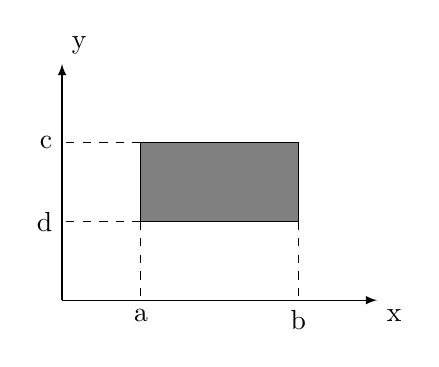
\begin{tikzpicture}
        \draw[-latex] (0,0) -- (4,0) node[below right]{x};
        \draw[-latex] (0,0) -- (0,3) node[above right]{y};
        \draw[fill = gray] (1,1) rectangle (3,2);
        \draw[dashed] (1,1) -- (1,0) node[below]{a};
        \draw[dashed] (3,1) -- (3,0) node[below]{b};
        \draw[dashed] (1,2) -- (0,2) node[left]{c};
        \draw[dashed] (1,1) -- (0,1) node[left]{d};
      \end{tikzpicture}
    \end{center}

    同样的,$A \times B \times C$表示的是空间中的一个立方体,这里就不画了(邪恶的tikz).
  }%卡氏积的图示结尾

  \subsubsection{n维卡氏积}{
    \begin{itemize}
      \item n维卡氏积 : $$
              A_1 \times A_2 \times \dots \times A_n = \set{<x_1,x_2,\dots,x_n> | x_1 \in A_1 \land x_2 \in A_2 \land \dots \land x_n \in A_n}
            $$
      \item $A^n = A \times A \times \dots \times A$
      \item $\absoluteValue{A_i} = n_i,i = 1,2,\dots,n \Rightarrow \absoluteValue{A_1 \times A_2 \times \dots \times A_n} = n_1 \times n_2 \times \dots \times n_n$.
      \item n维卡氏积性质于2维卡氏积类似.
    \end{itemize}
  }%n维卡氏积结尾

  \subsubsection{n维卡氏积的性质}{
    \begin{itemize}
      \item 非交换 : $A \times B \times C \neq B \times C \times A$\ (要求$A,B,C$均非空,且互不相等)
      \item 非结合 : (非二元运算)
      \item 分配律 : 例如 : $A \times B \times (C \unionSet D) = (A \times B \times C) \unionSet (A \times B \times D)$
      \item 其他 : 比如$A \times B \times C = \emptyset \Leftrightarrow A = \emptyset \lor B = \emptyset \lor C = \emptyset$.
    \end{itemize}
  }%n维卡氏积的性质结尾

}%有序对与卡氏积结尾

\subsection{二元关系}{

  \subsubsection{n元关系}{
    \begin{itemize}
      \item n元关系 : 其元素全是有序n元组的集合.
      \item 例1 : $F_1 = \set{<a,b,c,d>,<1,2,3,4>,<\alpha,\beta,\gamma,\delta>}$---$F_1$是3元关系.
      \item 例2 : $F_2 = \set{<a,b,c>,<\alpha,\beta,\gamma>,<A,B,C>}$---$F_2$是3元关系
    \end{itemize}
  }%n元关系结尾

  \subsubsection{二元关系}{
    \begin{itemize}
      \item 2元关系(关系) : 元素全是有序对的集合.
      \item 比如$A = \set{<A,B>,<1,2,3>,a,\alpha,1}$---如果$a,\alpha,1$不是有序对,那么$A$不是关系.
    \end{itemize}
  }%二元关系结尾

  \subsubsection{二元关系的记号}{
    \begin{itemize}
      \item{
            设$F$是二元关系,那么有三种记法 :

            \begin{itemize}
              \item 中缀(infix)记号 : $xFy$
              \item 前缀(prefix)记号 : $F(x,t),Fxy$
              \item 后缀(suffix)记号 : $\dependent{,xy} \in F,xyF$
            \end{itemize}
            }
      \item 例如 : $2 < 15 \Leftrightarrow <(2,15) \Leftrightarrow \dependent{2,15} \in <$
    \end{itemize}
  }%二元关系的记号结尾

  \subsubsection{A到B的二元关系}{
    \begin{itemize}
      \item {
            A到B的二元关系 : 是$A \times B$的任意子集.

            $R$是$A$到$B$的二元关系$\Leftrightarrow R \subseteq A \times B \Leftrightarrow R \in \powerSetOf{A \times B}$
            }
      \item 如果$\absoluteValue{A} = m,\absoluteValue{B} = n$,则$\absoluteValue{A \times B} = mn$,所以$\absoluteValue{P(A \times B)} = 2^{mn}$,也就是说$A$到$B$不同的二元关系共有$2^{mn}$个.
    \end{itemize}
  }%A到B的二元关系结尾

  \subsubsection{A到B的二元关系举例}{
    设$A = \set{a_1,a_2},B = \set{b_1,b_2}$,则$A$到$B$的二元关系共有4个 : $$
      R_1 = \emptyset,R_2 = \set{\dependent{a_1,b}},R_3 = \set{\dependent{a_2,b}},R_4 = \set{\dependent{a_1,b},\dependent{a_2,b}}
    $$

    反过来,$B$到$A$的二元关系也有4个 : $$
      R_5 = \emptyset.R_6 = \set{\dependent{b,a_1}},R_7 = \set{\dependent{b,a_2}},R_8 = \set{\dependent{b,a_1},\dependent{b,a_2}}
    $$
  }%A到B的二元关系举例结尾

  \subsubsection{A上的二元关系}{
    \begin{itemize}
      \item {
            $A$上的二元关系 : 是$A \times A$的任意子集.

            $R$是$A$上的二元关系 $\Leftrightarrow R \subseteq A \times A \Leftrightarrow R \in P(A \times A)$
            }
      \item {
            如果$\absoluteValue{A} = m$,则$\absoluteValue{A \times A} = m^2$,所以 : $$
              \absoluteValue{P(A \times A)} = 2^{m^2}
            $$

            即$A$上不同的二元关系共有$2^{m^2}$个
            }
    \end{itemize}
  }%A上的二元关系

  \subsubsection{一些特殊关系}{
    \begin{itemize}
      \item {
            设$A$是任意集合,则可以定义$A$上的 :

            \begin{itemize}
              \item 空关系 : $\emptyset$
              \item 恒等关系 : $I_A = \set{\dependent{x,x}| x \in A}$
              \item 全域关系 : $E_A = A \times A = \set{\dependent{x,y} | x \in A \land y \in A}$
              \item 包含关系 : $\subseteq_A = \set{\dependent{x,y}|x \subseteq \land y \subseteq A \land x \subseteq y}$
              \item 真包含关系 : $\subset_A = \set{\dependent{x,y} | x \subseteq A \land y \subseteq A \land x \subset y}$
            \end{itemize}
            }
      \item {
            设$A \subseteq Z$,则可以定义$A$上的 :

            \begin{itemize}
              \item 整除关系 : $D_A = \set{\dependent{x,y} | x \in A \land y \in A \land x|y}$
              \item {
                    例 : $A = \set{1,2,3,4}$,则 : $$
                      D_A = \set{\dependent{1,1},\dependent{1,2},\dependent{1,3},\dependent{1,4},\dependent{2,2},\dependent{2,4},\dependent{3,3},\dependent{4,4}}
                    $$
                    }
            \end{itemize}
            }
      \item {
            设$A \subset R$,则可以定义$A$上的 :

            \begin{itemize}
              \item 小于等于(less than or equal to)关系 : $LE_A = \set{\dependent{x,y}|x \in A \land y \in A \land x \leq y}$
              \item 小于(less than)关系 : $L_A = \set{\dependent{x,y}| x \in A \land y \in A \land x < y}$
              \item 大于等于(greater than or equal to)关系
              \item 大于(greater than)关系,\dots
            \end{itemize}
            }
    \end{itemize}
  }%一些特殊关系结尾

  \subsubsection{与二元关系有关的概念}{
    \begin{itemize}
      \item {
            对任意集合$R$,可以定义 :

            \begin{itemize}
              \item 定义域(domain) : $dom\ R = \set{x | \exists y(x R y)}$
              \item 值域(range) : $ran\ R = \set{y | \exists x(x R y)}$
              \item 域(field) : $fld\ R = dom\ R \unionSet ran\ R$
            \end{itemize}

            例 : \begin{itemize}
              \item $R_1 = \set{a,b}$
              \item $R_2 = \set{a,b,\dependent{c,d},\dependent{e,f}}$
              \item $R_3 = \set{\dependent{1,2}, \dependent{3,4}, \dependent{5,6}}$
            \end{itemize}

            当$a,b$不是有序对时,$R_1$和$R_2$不是关系.
            \begin{itemize}
              \item $dom\ R_1 = \emptyset,ran\ R_1 = \emptyset,fld\ R_1 = \emptyset$
              \item $dom\ R_2 = \set{c,e}, ran\ R_2 = \set{d,f},fld\ R_2 = \set{c,d,e,f}$
              \item $dom\ R_3 = \set{1,3,5}, ran\ R_3 = \set{2,4,6}, fld\ R_3 \set{1,2,3,4,5,6}$
            \end{itemize}
            }
      \item {
            对任意集合$F,G$,可以定义 :

            \begin{itemize}
              \item {
                    逆(inverse) : $F\inverse = \set{\dependent{x,y} | yFx}$

                    定理 : 设$F,G$为二集合,则$(F \circ G)\inverse = G\inverse \circ F\inverse$

                    这个可以用矩阵的逆来理解.

                    证明 : \begin{math}
                      \forall \dependent{x,y},\dependent{x,y} \in (F \circ G)\inverse \\
                      \Leftrightarrow \dependent{y,x} \in (F \circ G) \\
                      \Leftrightarrow \exists z (yGz \land zFx) \\
                      \Leftrightarrow \exists z (z G\inverse y \land x F\inverse z) \\
                      \Leftrightarrow \exists z (x F\inverse z \land z G\inverse y) \Leftrightarrow \dependent{x,y} \in G\inverse \circ F\inverse
                    \end{math}

                    \qed
                    }
              \item {
                    合成(复合)(composite) : $F \circ G = \set{\dependent{x,y} | \exists z(xGz \land zFy)}$

                    \begin{center}
                      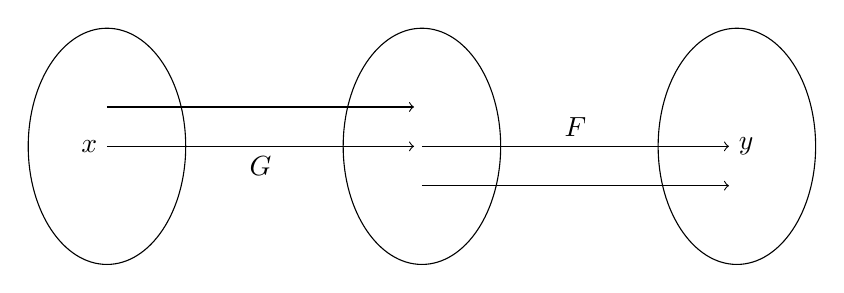
\begin{tikzpicture}
                        \draw (-4,0) ellipse [x radius = 1,y radius = 1.5];
                        \draw (0,0) ellipse [x radius = 1,y radius = 1.5];
                        \draw (4,0) ellipse [x radius = 1,y radius = 1.5];
                        \foreach \xOffset in {-4,0,4}{
                            \foreach \yOffset in {0.5,0,-0.5}{
                                \tikzPlaceDot{(\xOffset,\yOffset)};
                              }
                          }
                        \draw[->] (-4,0.5) -- (-0.1,0.5);
                        \draw[->] (-4,0) node[left]{$x$} --node[below]{$G$} (-0.1,0);
                        \draw[->] (0,0) --node[above]{$F$} (3.9,0) node[right]{$y$};
                        \draw[->] (0,-0.5) -- (3.9,-0.5);
                      \end{tikzpicture}
                    \end{center}

                    关于合成,还分为 :

                    \begin{itemize}
                      \item 顺序合成(右合成) : $F \circ G = \set{\dependent{x,y} | \exists z (xFz \land zGy)}$
                      \item 逆序合成(左合成) : $F \circ G = \set{\dependent{x,y} | \exists z (xGz \land zFy)}$
                    \end{itemize}

                    合成运算有结合律 :

                    \begin{itemize}
                      \item 设$R_1,R_2,R_3$为集合,则 : $$
                              (R_1 \circ R_2) \circ R_3 = R_1 \circ (R_2 \circ R_3)
                            $$
                    \end{itemize}

                    证明 : \begin{math}
                      \forall\dependent{x,y}, \dependent{x,y} \in (R_1 \circ R_2) \circ R_3 \\
                      \Leftrightarrow \exists z (x R_3 z \land z(R_1 \circ R_2)y) \\
                      \Leftrightarrow \exists z (x R_3 z \land \exists t(z R_2 t \land t R_1 y)) \\
                      \Leftrightarrow \exists z \exists t(x R_3 z \land (z R_2 t \land t R_1 y)) \\
                      \Leftrightarrow \exists t \exists z(x R_3 z \land z R_2 t \land t R_1 y) \\
                      \Leftrightarrow \exists t \exists z (x R_3 z \land z R_2 t \land t R_1 y) \\
                      \Leftrightarrow \exists t(\exists z(x R_3 z \land z R_2 t) \land t R_1 y) \\
                      \Leftrightarrow \exists t(x(R_2 \circ R_3)t \land t R_1 y) \\
                      \Leftrightarrow x R_1 \circ (R_2 \circ R_3) y \\
                      \Leftrightarrow \dependent{x,y} \in R_1 \circ (R_2 \circ R_3) \\
                      \therefore (R_1 \circ R_2) \circ R_3 = R_1 \circ (R_2 \circ R_3)
                    \end{math}

                    \qed
                    }
            \end{itemize}
            }
      \item {
            对任意集合$F,A$,可以定义 :

            \begin{itemize}
              \item 限制(restriction) : $F \upharpoonright  A = \set{\dependent{x,y} | xFy \land x \in A}$
              \item 象(image) : $F[A] = ran(F \upharpoonright A),F[A] = \set{y | \exists x (x \in A \land xFy)}$
            \end{itemize}
            }
      \item {
            对任意集合$F$,可以定义 :

            \begin{itemize}
              \item {
                    单根(single rooted) : 一个$y$对应唯一的一个$x$就是单根.

                    $F$是单根的 $\Leftrightarrow \forall y(y \in ran\ F \to \exists! x(x \in dom\ F \land xFy)) \Leftrightarrow (\forall y \in ran\ F)(\exists! x \in dom\ F)(xFy)$

                    \begin{itemize}
                      \item $\exists!$表示"存在唯一的"
                      \item $\forall x (x \in A \to B(x))$缩写为$(\forall x \in A)B(x)$
                      \item $\exists x (x \in A \land B(x))$缩写为$(\exists x \in A)B(x)$
                    \end{itemize}
                    }
              \item {
                    单值(single valued) : 一个$x$对应一个唯一的$y$就是单值.
                    $$
                      \mbox{$F$是单值的} \Leftrightarrow \forall x(x \in dom\ F \to \exists! y (y \in \rangle F \land xFy)) \Leftrightarrow (\forall x \in dom\ F)(\exists! y \in ran\ F)(xFy)
                    $$
                    }
            \end{itemize}
            }
    \end{itemize}
  }%与二元关系有关的概念结尾

}%二元关系结尾

\subsection{关系的表示与性质}{

  \subsubsection{关系矩阵}{
    设$A = \set{a_1,a_2,...,a_n},R \subseteq A \times A$

    $R$的关系矩阵为一个$n \times n$的方阵$M(R) = (r_{ij})_{n \times n}$ : $$
      M(R)(i,j) = r_{ij} = \begin{cases}
        1,\ a_iRa_j \\
        0,\ \mbox{否则}
      \end{cases}
    $$

    举个例子 : \begin{itemize}
      \item $A = \set{a,b,c}$
      \item $R_1 = \set{\dependent{a,a},\dependent{a,b},\dependent{b,a},\dependent{b,c}}$
      \item $R_2 = \set{\dependent{a,b},\dependent{a,c},\dependent{b,c}}$
    \end{itemize}

    $$
      M(R_1) = \begin{bmatrix}
        1 & 1 & 0 \\
        1 & 0 & 1 \\
        0 & 0 & 0
      \end{bmatrix}
      \qquad
      M(R_2) = \begin{bmatrix}
        0 & 1 & 1 \\
        0 & 0 & 1 \\
        0 & 0 & 0
      \end{bmatrix}
    $$

    注 : 默认从左到右,从上到下按$a,b,c$的顺序排列.
  }%关系矩阵结尾

  \subsubsection{关系矩阵的性质}{
    \begin{itemize}
      \item 集合表达式与关系矩阵可以唯一互相确定
      \item $M(R\inverse) = (M(R))\transpose$\begin{itemize}
              \item $~\transpose$表示矩阵转置
            \end{itemize}
      \item $M(R_1 \circ R_2) = M(R_2) \cdot M(R_1)$\begin{itemize}
              \item $\cdot$表示矩阵的"逻辑乘"(即分量相加或数乘换成逻辑操作),加法用$\lor$,乘法用$\land$
            \end{itemize}
    \end{itemize}
  }%关系矩阵的性质结尾

  \subsubsection{关系矩阵举例}{
    \begin{itemize}
      \item $A = \set{a,b,v}$
      \item $R_1 = \set{\dependent{a,a},\dependent{a,b},\dependent{b,a},\dependent{b,c}}$
      \item $R_2 = \set{\dependent{a,b},\dependent{a,c},\dependent{b,c}}$
      \item 用$M(R_1),M(R_2)$确定$M(R_1\inverse),M(R_2\inverse),M(R_1 \circ R_1),M(R_1 \circ R_2)$,从而求出他们的集合表达式.
    \end{itemize}

    解 : $$
      M(R_1) = \begin{bmatrix}
        1 & 1 & 0 \\
        1 & 0 & 1 \\
        0 & 0 & 0
      \end{bmatrix},\qquad
      M(R_2) = \begin{bmatrix}
        0 & 1 & 1 \\
        0 & 0 & 1 \\
        0 & 0 & 0
      \end{bmatrix},\qquad
      M(R_1\inverse) = \begin{bmatrix}
        1 & 1 & 0 \\
        1 & 0 & 0 \\
        0 & 1 & 0
      \end{bmatrix},\qquad
      M(R_2\inverse) = \begin{bmatrix}
        0 & 0 & 0 \\
        1 & 0 & 0 \\
        1 & 1 & 0
      \end{bmatrix}
    $$
    \begin{itemize}
      \item $R_1\inverse = \set{\dependent{a,a},\dependent{a,b},\dependent{b,a},\dependent{c,b}}$
      \item $R_2\inverse = \set{\dependent{b,a},\dependent{c,a},\dependent{c,b}}$
    \end{itemize}
    $$
      M(R_1 \circ R_1) = \begin{bmatrix}
        1 & 1 & 0 \\
        1 & 0 & 1 \\
        0 & 0 & 0
      \end{bmatrix}
      \cdot
      \begin{bmatrix}
        1 & 1 & 0 \\
        1 & 0 & 1 \\
        0 & 0 & 0
      \end{bmatrix}
      =
      \begin{bmatrix}
        1 & 1 & 1 \\
        1 & 1 & 0 \\
        0 & 0 & 0
      \end{bmatrix}
    $$
    \begin{itemize}
      \item $R_1 \circ R_1 = \set{\dependent{a,a},\dependent{a,b},\dependent{a,c},\dependent{b,a},\dependent{b,b}}$
    \end{itemize}
    $$
      M(R_1 \circ R_2) = \begin{bmatrix}
        0 & 1 & 1 \\
        0 & 0 & 1 \\
        0 & 0 & 0
      \end{bmatrix}
      \cdot
      \begin{bmatrix}
        1 & 1 & 0 \\
        1 & 0 & 1 \\
        0 & 0 & 0
      \end{bmatrix}
      =
      \begin{bmatrix}
        1 & 0 & 1 \\
        0 & 0 & 0 \\
        0 & 0 & 0
      \end{bmatrix}
    $$
    \begin{itemize}
      \item $R_1 \circ R_2 = \set{\dependent{a,a},\dependent{a,c}}$
    \end{itemize}
  }%关系矩阵举例结尾

  \subsubsection{关系图}{
    \begin{itemize}
      \item $A = \set{a_1,a_2,\dots,a_n},R \subseteq A \times A$
      \item {
            $R$的关系图$G(R)$ : \begin{itemize}
              \item 以"$o$"表示$A$中元素(称为顶点), 以"$\rightarrow$"表示$R$中元素(称为有向边)
              \item 若$a_iRa_j$,则从顶点$a_i$向顶点$a_j$引有向边$\dependent{a_i,a_j}$
            \end{itemize}
            }
    \end{itemize}
  }%关系图结尾

  \subsubsection{关系图举例}{
    \begin{itemize}
      \item $A = \set{a,b,c}$
      \item $R_1 = \set{\dependent{a,a},\dependent{a,b},\dependent{b,a},\dependent{b,c}}$
      \item $R_2 = \set{\dependent{a,b},\dependent{a,c},\dependent{b,c}}$
      \item $R_1\inverse = \set{\dependent{a,a},\dependent{a,b},\dependent{b,a},\dependent{c,b}}$
      \item $R_2\inverse = \set{\dependent{b,a},\dependent{c,a},\dependent{c,b}}$
      \item $R_1 \circ R_1 = \set{\dependent{a,a},\dependent{a,b},\dependent{a,c},\dependent{b,a},\dependent{b,b}}$
      \item $R_1 \circ R_1 = \set{\dependent{a,a},\dependent{a,c}}$
      \item $R_2 \circ R_1 = \set{\dependent{a,b},\dependent{a,c},\dependent{b,b},\dependent{b,c}}$
    \end{itemize}
    \begin{center}
      \includegraphics[scale=0.5]{resources/dependGraphic_1.png}

      去他妈的tikz!
    \end{center}
  }%关系图举例

  \subsubsection{讨论}{
    \begin{itemize}
      \item 当$A$中元素标定次序后,对于$R \subseteq A \times A$ : \begin{itemize}
              \item $G(R)$与$R$的集合表达式可唯一互相确定.
              \item $R$的集合表达式,关系矩阵,关系图三者均可唯一互相确定.
            \end{itemize}
      \item 对于$R \subseteq A \times B$ : \begin{itemize}
              \item $\absoluteValue{A} = n,\absoluteValue{B} = m$,关系矩阵$M(R)$时$n \times m$阶.
              \item $G(R)$中边都是从$A$中元素指向$B$中元素.
            \end{itemize}
    \end{itemize}
  }%讨论结尾

  \subsubsection{关系的性质}{
    \begin{itemize}
      \item {
            自反性(reflexivity) : \begin{itemize}
              \item $R \subseteq A \times A$
              \item $R$是自反的$\Leftrightarrow \forall x(x \in A \to xRx) \Leftrightarrow (\forall x \in A)xRx$
              \item $R$是非自反的$\Leftrightarrow \exists x (x \in A \land \lnot xRx)$
            \end{itemize}

            \begin{center}
              \includegraphics{resources/reflexivity.png}
            \end{center}

            定理 : 以下描述等价
            \begin{itemize}
              \item $R$是自反的
              \item $I_A \subseteq R$
              \item $R\inverse$是自反的
              \item $M(R)$主对角线上的元素全为$1$
              \item $G(R)$的每个顶点处均有环.
            \end{itemize}
            }
      \item {
            反自反性(irreflexivity) : \begin{itemize}
              \item $R \subseteq A \times A$
              \item $R$是反自反的$\Leftrightarrow \forall x(x \in A \to \lnot xRx) \Leftrightarrow (\forall x \in A)\lnot xRx$
              \item $R$是非反自反的$\Leftrightarrow \exists x(x \in A \land xRx)$
            \end{itemize}

            \begin{center}
              \includegraphics{resources/irreflexivity.png}
            \end{center}

            定理 : 以下描述等价
            \begin{itemize}
              \item $R$是反自反的
              \item $I_A \intersectionSet R = \emptyset$
              \item $R\inverse$是反自反的
              \item $M(R)$主对角线上的元素全为0
              \item $G(R)$的每个顶点处均无环.
            \end{itemize}

            自反且反自反 : $\emptyset$上的空关系
            }
      \item {
            对称性(symmetry) : \begin{itemize}
              \item $R \subseteq A \times A$
              \item $R$是对称的$\Leftrightarrow \forall x \forall y (x \in A \land y \in A \land xRy \to yRx) \Leftrightarrow (\forall x \in A)(\forall y \in A)[xRy \to yRx]$
              \item $R$是非对称的$\Leftrightarrow \exists x \exists y(x \in A \land y \in A \land xRy \land \lnot yRx)$
            \end{itemize}

            \begin{center}
              \includegraphics{resources/symmetry.png}
            \end{center}

            定理 : 以下描述等价
            \begin{itemize}
              \item $R$是对称的
              \item $R\inverse = R$
              \item $R\inverse$是对称的
              \item $G(R)$的任何两个顶点之间若有边,则必有两条方向相反的有向边.
            \end{itemize}
            }
      \item {
            反对称性(antisymmetry) : \begin{itemize}
              \item $R \subseteq A \times A$
              \item $R$是反对称的$\Leftrightarrow \forall x \forall y(x \in A \land y \in A \land xRy \land yRx \to x = y) \Leftrightarrow (\forall x \in A)(\forall y \in A)[xRy \land yRx \to x = y]$
              \item $R$非反对称$\Leftrightarrow \exists x \exists y (x \in A \land y \in A \land xRy \land yRx \land x \neq y)$
            \end{itemize}

            \begin{center}
              \includegraphics{resources/antisymmetry.png}
            \end{center}

            定理 : 以下叙述等价
            \begin{itemize}
              \item $R$是反对称的
              \item $R\inverse \intersectionSet R \subseteq I_A$
              \item $R\inverse$是反对称的
              \item 在$M(R)$中,$\forall i \forall j(i \neq j \land r_{ij} = 1 \to r_{ji} = 0)$
              \item 在$G(R)$中,$\forall a_i \forall a_j (i \neq j)$,若有有向边$\dependent{a_i,a_j}$,则必没有$\dependent{a_j,a_i}$.
            \end{itemize}
            }
      \item {
            传递性(transivity) : \begin{itemize}
              \item $R \subseteq A \times A$
              \item $R$是传递的$\Leftrightarrow \forall x \forall y \forall z (x \in A \land y \in A \land z \in A \land xRy \land yRz \to xRz)\Leftrightarrow(\forall x \in A)(\forall y \in A)(\forall z \in A)[xRy \land yRz \to xRz]$
              \item $R$非传递$\Leftrightarrow \exists x \exists y \exists z (x \in A \land y \in A \land z \in A \land xRy \land yRz \land \lnot xRz)$
            \end{itemize}

            \begin{center}
              \includegraphics{resources/transivity.png}
            \end{center}

            定理 : 以下叙述等价
            \begin{itemize}
              \item $R$是传递的
              \item $R \circ R \subseteq R \Leftrightarrow R\inverse$是传递的
              \item $\forall i \forall j,M(R \circ R)(i,j) \leq M(R)(i,j)$
              \item 在$G(R)$中,$\forall a_i \forall a_j \forall a_k$,若有有向边$\dependent{a_i,a_j}$和$\dependent{a_j,a_k}$,则必有有向边$\dependent{a_i,a_k}$
            \end{itemize}
            }
    \end{itemize}

    在$\mathNatureNumberCollection = \set{0,1,2,...}$上 : \begin{itemize}
      \item $\leq = \set{\dependent{x,y} | x \in \mathNatureNumberCollection \land y \in \mathNatureNumberCollection \land x \leq y}$自反,反对称,传递
      \item $\geq = \set{\dependent{x,y} | x \in \mathNatureNumberCollection \land y \in \mathNatureNumberCollection \land x \geq y}$自反,反对称,传递
      \item $< = \set{\dependent{x,y} | x \in \mathNatureNumberCollection \land y \in \mathNatureNumberCollection \land x < y}$反自反,反对称,传递
      \item $> = \set{\dependent{x,y} | x \in \mathNatureNumberCollection \land y \in \mathNatureNumberCollection \land x > y}$反自反,反对称,传递
      \item $| = \set{\dependent{x,y} | x \in \mathNatureNumberCollection \land y \in \mathNatureNumberCollection \land x | y}$反对称,传递($\lnot 0 | 0$)
      \item $I_N = \set{\dependent{x,y} | x \in \mathNatureNumberCollection \land y \in \mathNatureNumberCollection \land x = y}$自反,对称,反对称,传递
      \item $E_N = \set{\dependent{x,y} | x \in \mathNatureNumberCollection \land y \in \mathNatureNumberCollection} = \mathNatureNumberCollection \times \mathNatureNumberCollection$自反,对称,传递
    \end{itemize}
  }%关系的性质结尾

}%关系的表示与性质结尾

\subsection{关系的幂运算和闭包}{

  \subsubsection{关系的n次幂}{
    \begin{itemize}
      \item {
            $R \subseteq A \times A,n \in \mathNatureNumberCollection$

            $$
              \begin{cases}
                R^0 = I_A \\
                R^{n + 1} = R^n \circ R\ (n \geq 0)
              \end{cases}
            $$
            }
      \item {
            显然$R^n \subseteq A \times A,n \in \mathNatureNumberCollection$
            }
    \end{itemize}

    $$
      R^n = R \circ R \circ \dots \circ R\qquad(n\mbox{个}R)
    $$

  }%关系的n次幂结尾

  \subsubsection{关系的幂运算的一些定理}{
    设$R \subseteq A \times A,m,n \in \mathNatureNumberCollection$,则 : \begin{enumerate}
      \item $R^m \circ R^n = R^{m + n}$
      \item $(R^m)^n = R^{mn}$
    \end{enumerate}

    \begin{proof}
      \begin{enumerate}
        \item {
              给定$m$,对$n$归纳 : $n = 0$时 : $$
                R^m \circ R^n = R^m \circ R^0 = R^m \circ I_A = R^m = R^{m + 0}
              $$

              假设$R^m \circ R^n = R^{m + n}$,则 :
              \begin{math}
                R^m \circ R^{n + 1} \\
                = R^m \circ (R^n \circ R^1) \\
                = (R^m \circ R^n) \circ R^1 \\
                = R^{m + n} \circ R \\
                = R^{(m + n) + 1} \\
                = R^{m + (n + 1)}
              \end{math}
              }
        \item 可类似证明.
      \end{enumerate}
    \end{proof}

    一言以蔽之,指数律对关系的幂运算也成立.
  }%关系的幂运算的一些定理结尾

  \subsubsection{幂运算举例}{
    尚未参透tikz怎么玩,就先拿ppt糊一下.

    \begin{center}
      \includegraphics{resources/depend_power_example_1.png}
      \includegraphics{resources/depend_power_example.png}
    \end{center}
  }

  思考:这好像和隔壁教线代的GS老爷子的骚操作有点关系...
}%关系的幂运算和闭包结尾

\subsubsection{关系的闭包}{
  在数学上,闭包的定义一般指的是这个意思 : 包含给定的一些元素,并且具有某种指定性质的最小集合称为 : 某些元素具有某性质的闭包.

  所以闭包一般有三个性质 : \begin{enumerate}
    \item 包含给定的元素
    \item 具有给定的性质
    \item 是最小的二元关系
  \end{enumerate}

  其中关系的闭包主要有以下三种 :

  \begin{itemize}
    \item 自反闭包$r(R)$ : 包含$R$,向$R$中加一些元素,使$R$自反.
    \item 对称闭包$s(R)$ : 包含$R$,并且使$R$对称.
    \item 传递闭包$t(R)$ : 包含$R$,并且使$R$构成传递的二元关系.
  \end{itemize}
}%关系的闭包

\subsubsection{自反闭包}{
  自反闭包$r(R)$有以下性质(定义也如下) : \begin{enumerate}
    \item $R \subseteq r(R)$
    \item $r(R)$是自反的
    \item $\forall s ((R \subseteq S \land S\mbox{自反}) \to r(R) \subseteq S)$ 注 : 此条是所谓"最小的"的其中一种定义.
  \end{enumerate}

  \begin{center}
    \includegraphics{resources/Reflexive_closure.png}
  \end{center}
}%自反闭包结尾

\subsubsection{对称闭包}{
  对称闭包有以下性质(定义也如下) : \begin{enumerate}
    \item $R \subseteq s(R)$
    \item $s(R)$是对称的
    \item $\forall S ((R \subseteq S \land S\mbox{对称}) \to s(R) \subseteq S)$ 注 : 此条是所谓"最小的"的其中一种定义.
  \end{enumerate}

  \begin{center}
    \includegraphics{resources/Symmetric_closure.png}
  \end{center}
}%对称闭包结尾

\subsubsection{传递闭包}{
  传递闭包有以下性质(定义也如下) : \begin{enumerate}
    \item $R \subseteq t(R)$
    \item $t(R)$是传递的
    \item $\forall S ((R \subseteq S \land S\mbox{传递}) \to t(R) \subseteq S)$ 注 : 此条是所谓"最小的"的其中一种定义.
  \end{enumerate}

  \begin{center}
    \includegraphics{resources/transivity_closure.png}
  \end{center}
}%传递闭包结尾

\subsubsection{关于闭包的一些定理}{
  \begin{enumerate}
    \item {
          设$R \subseteq A \times A$且$A \neq \emptyset$,则 : \begin{enumerate}
            \item $R$自反$\Leftrightarrow r(R) = R$
            \item $R$对称$\Leftrightarrow s(R) = R$
            \item $R$传递$\Leftrightarrow t(R) = R$
          \end{enumerate}
          }
    \item {
          设$R_1 \subseteq R_2 \subseteq A \times A$且$A \neq \emptyset$,则 : \begin{enumerate}
            \item $r(R_1) \subseteq r(R_2)$
            \item $s(R_1) \subseteq s(R_2)$
            \item $t(R_1) \subseteq t(R_2)$
          \end{enumerate}
          }
    \item {
          设$R_1,R_2\subseteq A \times A$且$A \neq \emptyset$,则 : \begin{enumerate}
            \item $r(R_1 \unionSet R_2) = r(R_1) \unionSet r(R_2)$
            \item $s(R_1 \unionSet R_2) = s(R_1) \unionSet s(R_2)$
            \item $t(R_1 \unionSet R_2) \supseteq t(R_1) \unionSet t(R_2)$
          \end{enumerate}
          \begin{proof}
            如下 :

            \begin{enumerate}
              \item {
                    $R_1 \unionSet R_2 \subseteq r(R_1) \unionSet r(R_2) \subseteq r(R_1 \unionSet R_2)$

                    又由$r(R_1) \unionSet r(R_2)$自反,所以$r(R_1 \unionSet R_2) \subseteq r(R_1) \unionSet r(R_2)$
                    }
              \item 可类似证明
              \item $t(R_1) \unionSet t(R_2) \subseteq t(R_1 \unionSet R_2)$
            \end{enumerate}
          \end{proof}
          注 : $t(R_1) \unionSet t(R_2)$不一定传递,反例如下 :

          \begin{center}
            \includegraphics{resources/transivity_closure_2.png}
          \end{center}
          }
  \end{enumerate}
}%关于闭包的一些定理结尾

\subsubsection{闭包的求法}{
  \begin{itemize}
    \item 设$R \subseteq A \times A$且$A \neq \emptyset$,则 : \begin{itemize}
            \item $r(R) = R \unionSet I_A$(图形表示就是给每个点加上环)
            \item $s(R) = R \unionSet R\inverse$(图形表示就是给每个边加上反向的边)
            \item $t(R) = R \unionSet R^2 \unionSet R^3 \unionSet \dots$(传递闭包)
          \end{itemize}
    \item 对比 : \begin{itemize}
            \item $R$自反$\Leftrightarrow I_A \subseteq R$
            \item $R$对称$\Leftrightarrow R = R\inverse$
            \item $R$传递$\Leftrightarrow R^2 \subseteq R$
          \end{itemize}
  \end{itemize}

  \begin{proof}
    设$R \subseteq A \times A$且$A \neq \emptyset$,则 : \begin{itemize}
      \item {
            $r(R) = R \unionSet I_A$

            证明如下 :\begin{enumerate}
              \item $R \subseteq R \unionSet I_A$
              \item $I_A \subseteq R \unionSet I_A \Leftrightarrow R \unionSet I_A$自反$\Rightarrow r(R) \subseteq R \unionSet I_A$
              \item $R \subseteq r(R) \land r(R)$自反$\Rightarrow R \subseteq r(R) \land I_A \subseteq r(R) \Rightarrow R \unionSet I_A \subseteq r(R)$
            \end{enumerate}
            }
      \item {
            $s(R) = R \unionSet R\inverse$

            证明如下 : \begin{enumerate}
              \item $R \subseteq R \unionSet R\inverse$
              \item $(R \unionSet R\inverse)\inverse = R \unionSet R\inverse \Leftarrow R \unionSet R\inverse$对称$\Rightarrow s(R) \subseteq R \unionSet R\inverse$
              \item $R \subseteq s(R) \land R\inverse \subseteq s(R) \Rightarrow R \unionSet R\inverse \subseteq s(R)$
            \end{enumerate}
            }
      \item {
            $t(R) = R \unionSet R^2 \unionSet R^3 \unionSet \dots$

            证明如下 : \begin{enumerate}
              \item $R \subseteq R \unionSet R^2 \unionSet R^3 \unionSet \dots$
              \item {
                    \begin{itemize}
                      \item[] $(R \unionSet R^2 \unionSet R^3 \unionSet \dots)^2$
                      \item[$=$] $R^2 \unionSet R^3 \unionSet \dots \subseteq R \unionSet R^2 \unionSet R^3 \unionSet \dots$
                      \item[$\Leftrightarrow$]这玩意传递
                      \item[$\Rightarrow$] $t(R) \subseteq R \unionSet R^2 \unionSet R^3 \unionSet \dots$
                    \end{itemize}
                    }
              \item {
                    \begin{itemize}
                      \item[] $R \subseteq t(R) \land t(R)$传递
                      \item[$\Rightarrow$] $R \subseteq t(R) \land R^2 \subseteq t(R) \land R^3 \subseteq t(R) \land \dots$
                      \item[$\Rightarrow$] $R \unionSet R^2 \unionSet R^3 \unionSet \dots \unionSet \subseteq t(R)$
                    \end{itemize}

                    推论 : 设$R \subseteq A \times A$且$0 < \absoluteValue{A} < \absoluteValue{\infty}$,则$\exists I \in \mathNatureNumberCollection$,使得$t(R) = R \unionSet R^2 \unionSet R^3 \unionSet \dots \unionSet R^I$
                    }
            \end{enumerate}
            }
    \end{itemize}
  \end{proof}
}%闭包的求法结尾

\subsubsection{闭包运算与关系性质}{
  下表表示闭包运算后原本的关系的性质是否保持 :

  \begin{center}
    \begin{tabular}{|c|c|c|c|}
      \hline
      ~      & 自反性 & 对称性 & 传递性 \\
      \hline
      $r(R)$ & yes    & yes    & yes    \\
      \hline
      $s(R)$ & yes    & yes    & no     \\
      \hline
      $t(R)$ & yes    & yes    & yes    \\
      \hline
    \end{tabular}
  \end{center}

  以下为证明 :

  \begin{enumerate}
    \item {
          \begin{proof}
            $R$自反$\Rightarrow s(R)$和$t(R)$自反

            \begin{itemize}
              \item $I_A \subseteq R \unionSet R\inverse = s(R) \Rightarrow s(R)$自反
              \item $I_A \subseteq R \unionSet R^2 \unionSet R^3 \unionSet \dots t(R) \Rightarrow t(R)$自反
            \end{itemize}
          \end{proof}
          }
    \item {
          \begin{proof}
            $R$对称$\Rightarrow r(R)$和$t(R)$对称

            \begin{itemize}
              \item $r(R)\inverse = (I_A \unionSet R)\inverse = I_A\inverse \unionSet R\inverse = I_A \unionSet R\inverse = I_A \unionSet R = r(R) \Rightarrow r(R)$对称.
              \item {
                    \begin{itemize}
                      \item[] $t(R)\inverse = (R \unionSet R^2 \unionSet R^3 \unionSet \dots)\inverse$
                      \item[$=$] $R\inverse \unionSet (R^2)\inverse \unionSet (R^3)\inverse \unionSet \dots$
                      \item[$=$] $R\inverse \unionSet (R\inverse)^2 \unionSet (R\inverse)^3 \unionSet \dots$
                      \item[$=$] $R \unionSet R^2 \unionSet R^3 \unionSet \dots$
                      \item[$=$] $t(R)$
                      \item[$\Rightarrow$] $t(R)$对称.
                    \end{itemize}
                    }
            \end{itemize}
          \end{proof}
          }
    \item {
          \begin{proof}
            $R$传递$\Rightarrow r(R)$传递

            \begin{itemize}
              \item[] $r(R) \circ r(R) = (I_A \unionSet R) \circ (I_A \unionSet R)$
              \item[$=$] $(I_A \circ I_A) \unionSet (I_A \circ R) \unionSet (R \circ I_A) \unionSet (R \circ R)$
              \item[$\subseteq$] $I_A \unionSet R \unionSet R \unionSet R = I_A \unionSet R = r(R)$
              \item[$\Rightarrow$] $r(R)$传递.
            \end{itemize}
          \end{proof}

          注 : $R$传递$ \nRightarrow s(R)$传递,反例 :
          \begin{center}
            \begin{tikzpicture}
              \tikzPlaceNode{a}{(-1,0)}{~};
              \tikzPlaceNode{b}{(1,0)}{~};
              \draw[very thick,->] (a) -- (b);
            \end{tikzpicture}
            \begin{tikzpicture}
              \tikzPlaceNode{a}{(-1,0)}{~};
              \tikzPlaceNode{b}{(1,0)}{~};
              \tikzPlaceShiftLeftRightArrow{a}{b}
            \end{tikzpicture}

            $H(R)$ \qquad $G(s(R))$
          \end{center}
          }
  \end{enumerate}
}%闭包运算与关系性质结尾

\subsubsection{闭包运算与关系性质相关定理}{
  \begin{itemize}
    \item {
          设$R \subseteq A \times A$且$A \neq \emptyset$,则 : \begin{enumerate}
            \item $rs(R) = sr(R)$
            \item $rt(R) = tr(R)$
            \item $st(R) = ts(R)$
          \end{enumerate}

          注 : $rs(R) = r(s(R))$

          证明 : \begin{enumerate}
            \item {
                  \begin{itemize}
                    \item[] $rs(R) = r(s(R) = r(R \unionSet R\inverse)) = I_A \unionSet (R \unionSet R\inverse)$
                    \item[$=$] $(I_A \unionSet R) \unionSet (I_A\inverse \unionSet R\inverse) = (I_A \unionSet r) \unionSet (I_A \unionSet R)\inverse$
                    \item[$=$] $r(R) \unionSet r(R)\inverse = s(r(R)) = sr(R)$
                  \end{itemize}
                  }
            \item {
                  \begin{itemize}
                    \item[] $rt(R) = r(t(R)) = r(R \unionSet R^2 \unionSet R^3 \unionSet \dots) = I_A \unionSet (R \unionSet R^2 \unionSet R^3 \unionSet \dots)$
                    \item[$=$] $(I_A \unionSet R)\unionSet(I_A \unionSet R \unionSet R^2) \unionSet (I_A \unionSet R \unionSet R^2 \unionSet R^3) \unionSet \dots$
                    \item[$=$] $(I_A \unionSet R) \unionSet (I_A \unionSet R)^2 \unionSet (I_A \unionSet R)^3 \unionSet \dots$
                    \item[$=$] $r(R) \unionSet r(R)^2 \unionSet r(R)^3 \unionSet \dots$
                    \item[$=$] $t(r(R)) = tr(R)$
                  \end{itemize}
                  }
            \item {
                  $st(R) \subseteq st(s(R)) = sts(R) = s(ts(R)) = ts(R)$

                  ($ts(R)$对称)

                  反例 : $st(R) \subset ts(R)$ :
                  }
          \end{enumerate}
          }
  \end{itemize}

  \begin{center}
    \includegraphics{resources/closure_properties_example_1.png}
  \end{center}
}%闭包运算与关系性质相关定理结尾

}%集合论结尾

\section{图论}{

  \subsection{图论的主要内容}{
    \begin{itemize}
      \item 研究对象 : 由顶点和边构成的图
      \item 研究思想 : 以集合论为基础,以图为工具,为各种二元关系建立模型
      \item 研究内容 : \begin{itemize}
              \item 图的基本概念 : 连通性,矩阵表示,带权图
              \item 欧拉图,哈密顿图 : 边和顶点的遍历
              \item 树 : 表示层级组织关系
              \item 平面图 : 判定,表示,性质
              \item 图的着色 : 各种调度问题的模型
              \item 独立集,支配集,覆盖集,匹配 : 各种应用问题
            \end{itemize}
    \end{itemize}
  }%图论的主要内容结尾

  \subsection{图论中的问题}{
    \begin{itemize}
      \item 什么是图?有哪些图?图有什么性质?
      \item 什么是欧拉图?什么是哈密顿图?
      \item 什么是树?如何用矩阵表示图?
      \item 什么是图的着色?
      \item 什么是支配集,独立集,覆盖,匹配?
      \item 什么是带权图?
    \end{itemize}
  }%图论中的问题结尾

 }%图论结尾

}%离散数学结尾